\section{Invertibility and Isomorphisms}
We see in this section that the inverse of a linear transformation is also linear. This result greatly aids us  in the study of \textit{inverses} of matrices. As one might expect from Section 2.3, the inverse of the left-multiplication transformation $L_A$ (when it exists) can be used to determine properties of the inverse of the matrix \textit{A}.

In the remainder of this section, we apply many of the results about invertibility to the concept of \textit{isomorphism}. We'll see that finite-dimensional vector spaces (over \textit{K}) of equal dimension may be identified.

\dfn{Inverse of a function}{
  Let \textit{V} and \textit{W} be vector spaces, and let $T : V \longrightarrow W$ be linear. A function $U : W \longrightarrow V$ is said to be an \textbf{inverse} of \textit{T} if $TU = I_W$ and $UT = I_V$. If \textit{T} has an inverse, then \textit{T} is said to be \textbf{invertible}. Moreover, if \textit{T} is invertible, then the inverse of \textit{T} is unique and is denoted by $T^{-1}$
}

The following facts hold for invertible functions \textit{T} and \textit{U}.
\begin{enumerate}
  \item $(TU)^{-1} = U^{-1} T^{-1}$
  \item $(T^{-1})^{-1} = T$; in particular, $T^{-1}$ is invertible.
  \item Let $T : V \longrightarrow W$ be a linear transformation, where \textit{V} and \textit{W} are finite-dimensional spaces of equal dimension. Then \textit{T} is invertible \textit{if and only if} rank(\textit{T}) $=$ dim(\textit{V}).
\end{enumerate}

\thm{}{
  Let \textit{V} and \textit{W} be vector spaces, and let $T : V \longrightarrow W$ be linear and invertible. Then $T^{-1} : W \longrightarrow V$ is linear.
}

\nt{
  It now follows immediately that if \textit{T} is a linear transformation between vector spaces of equal (finite) dimension, then the conditions of being invertible, one-to-one, and onto are all equivalent.
}

\dfn{Inverse of a matrix}{
  Let \textit{A} be a $n \times n$ matrix. Then \textit{A} is \textbf{invertible} if there exists and $n \times n$ matrix \textit{B} such that $AB = BA = I$.
}

\nt {
  If \textit{A} is invertible, then the matrix \textit{B} such that $AB = BA = I$ is unique. Moreover, the matrix \textit{B} is called the \textbf{inverse} of \textit{A} and is denoted by $A^{-1}$
}

\ex{inverse of a matrix}{
  It's easy to verify that the invese of
  \[
  \begin{pmatrix}
    5 & 7\\
    2 & 3\\
  \end{pmatrix}
  \qquad \text{ is } \qquad
  \begin{pmatrix}
    3 & -7\\
    -2 & 5\\
  \end{pmatrix}
  \]
}

At this point, we develop a number of results that relate the inverse of matrices to the inverses of linear transformations.

\mlemma{}{
  Let \textit{T} be an invertible linear transformation from \textit{V} to \textit{W}. Then \textit{V} is finite-dimensional \textit{if and only if} \textit{W} is finite-dimensional. In this case, dim(\textit{V}) $=$ dim(\textit{W}).
}

\thm{}{
  Let \textit{V} and \textit{W} be finite-dimensional vector spaces with ordered bases $\beta$ and $\gamma$, respectively. Let $T : V \longrightarrow W$ be linear. Then \textit{T} is invertible \textit{if and only if} $[T]_\beta^\gamma$ is invertible. Furthermore, $[T^{-1}]_\gamma^\beta = ([T]_\beta^\gamma)^{-1}$.
}

\cor{}{
  Let \textit{V} be a finite-dimensional vector space with and ordered basis $\beta$, and let $T : V \longrightarrow V$ be linear. Then \textit{T} is invertible \textit{if and only if} $[T]_\beta$ is invertible. Furthermore, $[T^{-1}]_\beta = ([T]_\beta)^{-1}$.
}

\cor{}{
  Let \textit{A} be an $n \times n$ matrix. Then \textit{A} is invertible \textit{if and only if} $L_A$ is invertible. Furthermore, $(L_A)^{-1} = L_{A^{-1}}$
}

The notion of invertibility may be used to formalize what we've been already observed, that is, that certain vector spaces strongly resemble one another except for the form of their vectors.

\dfn{Isomorphism}{
  Let \textit{V} and \textit{W} be vector spaces. We say that \textit{V} is \textbf{isomorphic} to \textit{W} if there exists a linear transformation $T : V \rightarrow W$ that's invertible. Such a linear transformation is called an \textbf{isomorphism} from \textit{V} onto \textit{W}.
}

\ex{Isomorphism}{
  Define $T : F^2 \rightarrow P_1(F)$ by $T(a_1, a_2) = a_1 + a_2x$. It's easily checked that \textit{T} us an Isomorphism; so $F^2$ is isomorphic to $P_1(F).$
}

\thm{}{
  Let \textit{V} and \textit{W} be finite-dimensional vector spaces (over the same field). Then \textit{V} is isomorphic to \textit{W} \textit{if and only if} dim(\textit{V}) $=$ dim(\textit{W}).
}

\cor{}{
  Let \textit{V} be a vector space over \textit{K}. Then \textit{V} is isomorphic to $K^n$ \textit{if and only if} dim(\textit{V}) $=$ n.
}

Up to this point, we have associated linear transformations with their matrix representations. We're now in a position to prove that, as a vector space, the collection of all linear transformations between two given vector spaces may be identified wiht the appropriate vector space of $m \times n$ matrices.

\thm{}{
  Let \textit{V} and \textit{W} be finite-dimensional vector spaces over \textit{K} of dimensions \textit{n} and \textit{m}, respectively, and let $\beta$ and $\gamma$ be ordered bases for \textit{V} and \textit{W}, respectively. Then the function $\Phi : \mathcal L(V,W) \rightarrow M_{m \times n}(K)$, defined by 
  \[\Phi(T) = [T]_\beta^\gamma\] for $T \in \mathcal L(V,W)$, is an isomorphism.
}

\cor{}{
  Let \textit{V} and \textit{W} be finite-dimensional vector spaces of dimensions \textit{n} and \textit{m}, respectively. Then $\mathcal L(V,W)$ is finite-dimensional of dimension \textit{mn}.
}

We conclude this section with a result that allows us to see more clearly the relationship between linear transformations defined on abstract finite-dimensional vector spaces and linear transformations from $K^n$ to $K^m$.

\dfn{Standard representation of V with respect to a basis}{
  Let $\beta$ be an ordered basis for an \textit{n}-dimensionsional vector space \textit{V} over the field \textit{K}. The \textbf{standard representation of V with respect to $\beta$} is the function $\phi_\beta : V \rightarrow k^n$ defined by \[\phi_\beta (x) = [x]_\beta\] for each $x \in V$.
}

\ex{inverse of a matrix}{
  Let $\beta = \{(1,0), (0,1)\}$ and $\gamma = \{(1,2), (3,4)\}$. It's easily observed that $\beta$ and $\gamma$ are ordered bases for $\mathbb R^2$. For $x = (1, -2)$, we have
  \[
    \phi_\beta(x) = [x]_\beta = 
    \begin{pmatrix}
      1\\
      -2\\
    \end{pmatrix}
  \qquad \text{ and } \qquad
  \phi_\gamma(x) = [x]_\gamma = 
  \begin{pmatrix}
    -5\\
    2\\
  \end{pmatrix}
  \]
}

We observed earlier that $\phi_\beta$ is a linear transformation. The next theorem tells us much more.

\thm{}{
  For any finite-dimensional vector space \textit{V} with ordered basis $\beta$, $\phi_\beta$ is an isomorphism
}

This theorem provides us with an alternate proof that an \textit{n}-dimensionsional vector space is isomorphic to $K^n$.

Let \textit{V} and \textit{W} be vector spaces of dimension \textit{n} and \textit{m}, respectively, and let $T : V \rightarrow W$ be a linear transformation. Define $A = [T]_\beta^\gamma$, where $\beta$ and $\gamma$ are arbitrary ordered bases of \textit{V} and \textit{W}, respectively. We're now able to use $\phi_\beta$ and $\phi_\gamma$ to study the relationship between the linear transformations \textit{T} and $L_A : K^n \rightarrow K^m$.

Let us first consider the next figure. Notice that there are two composites of linear transformations that map \textit{V} into $K^m$:

\begin{figure}[h!]
  \centering
  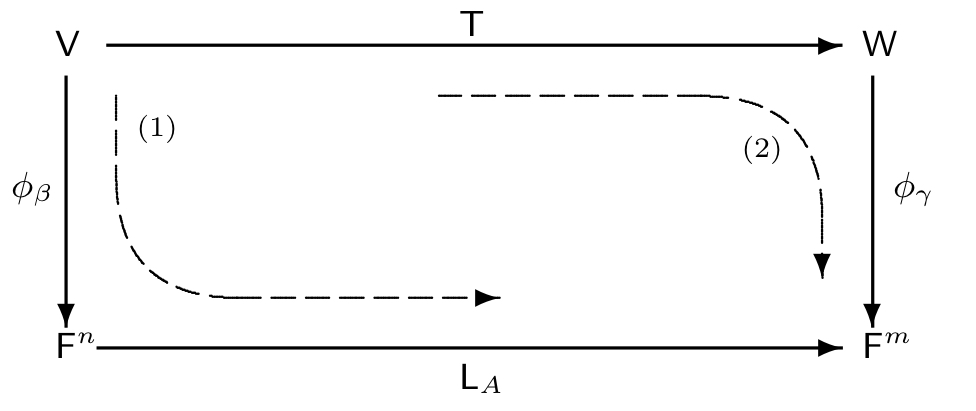
\includegraphics[width=0.7\textwidth]{invertibility-isomorphisms} 
\end{figure}

\begin{enumerate}
  \item Map \textit{V} into $K^n$ with $\phi_\beta$ and follow this transformation with $L_A$; this yields the composite $L_A \phi_\beta$.
  \item Map \textit{V} into \textit{W} with \textit{T} and follow it by $\phi_\gamma$ to obtain the composite $\phi_\gamma T$.
\end{enumerate}

These two composites are depicted by the dashed arrows in the diagram. Using an early theorem, we may conclude that 
\[L_A \phi_\beta = \phi_\gamma T;\]
that is, the diagram "commutes". Heuristically, the relationship indicates that after \textit{V} and \textit{W} are identified with $K^n$ and $K^m$ via $\phi_\beta$ and $\phi_\gamma$, respectively, we may "identiy" \textit{T} with $L_A$. This diagram allows us to transfer operations on abstract vector spaces to ones on $K^n$ and $K^m$.

\ex{}{
  Let the linear transformation $T : P_3(\mathbb R) \rightarrow P_2(\mathbb R)$ defined by $T(f(x)) = f'(x)$, $\beta$ and $\gamma$ be the standard ordered bases for $P_3(\mathbb R)$ and $P_2(\mathbb R)$, respectively, and let $\phi_\beta : P_3(\mathbb R) \rightarrow \mathbb R^4$ and $\phi_\gamma : P_2(\mathbb R) \rightarrow \mathbb R^3$ be the corresponding standard representations of $P_3(\mathbb R)$ and $P_2(\mathbb R)$. If $A = [T]_\beta^\gamma$, then
  \[
    A = 
    \begin{pmatrix}
      0 & 1 & 0 & 0\\
      0 & 0 & 2 & 0\\
      0 & 0 & 0 & 3\\
    \end{pmatrix}
  \]

  Consider the polynomial $p(x) = 2 + x - 3x^2 + 5x^3$. We show that $L_A \phi_\beta(p(x) = \phi_\gamma T(p(x))$. Now
  \[
    L_A \phi_\beta(p(x)) = 
    \begin{pmatrix}
      0 & 1 & 0 & 0\\
      0 & 0 & 2 & 0\\
      0 & 0 & 0 & 3\\
    \end{pmatrix}
    \begin{pmatrix}
      2\\
      1\\
      -3\\
      5\\
    \end{pmatrix}
    =
    \begin{pmatrix}
      1\\
      -6\\
      15\\
    \end{pmatrix}
  \]
But since $T(p(x)) = p'(x) = 1 - 6x + 15x^2$, we have
\[
  \phi_\gamma T(p(x)) =
  \begin{pmatrix}
    1\\
    -6\\
    15\\
  \end{pmatrix}
\]
So $L_A \phi_\beta(p(x) = \phi_\gamma T(p(x))$.
}
